\def\offset{2}
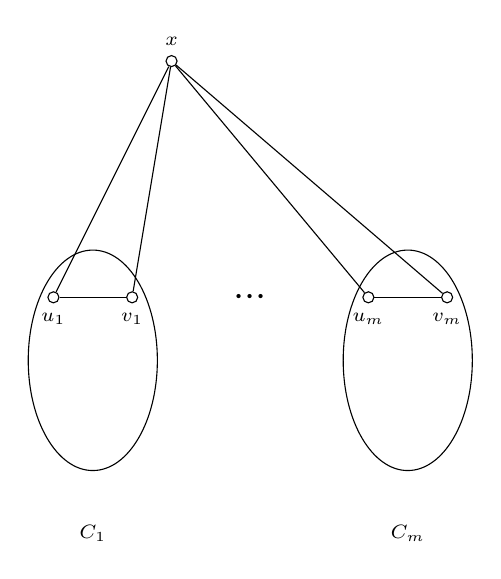
\begin{tikzpicture}

                \tikzstyle{vertex}  = [circle, minimum width=4pt, draw, inner sep=0pt, fill=white]
                \node [vertex, label=above:{\scriptsize$x$},](x) at (3.5, 6) {};

                \foreach \i in {1,2}
                {
                        \ifnum \i = 2
                                \node [vertex, label=below:{\scriptsize$u_m$}](u\i) at ({2 + \i * \offset}, 3) {};
                                \node [vertex, label=below:{\scriptsize$v_m$}](v\i) at ({3 + \i * \offset}, 3) {};
                                \node [minimum size=2.5cm, minimum width = 7pt](dots) at ({((2 + \i * \offset) - ( 1 + (\i-1) * \offset))*0.5 + ((1 + (\i-1) * \offset))}, 3) {\huge{$\scriptstyle \cdots$}};

                                \draw ({2 + \i * \offset + 0.5}, 2.2) ellipse (0.82cm and 1.4cm);
                                \node (c\i) at ({2 + \i * \offset + 0.5}, 0) {\scriptsize$C_m$};



                        \else
                                \node [vertex, label=below:{\scriptsize$u_\i$}](u\i) at ({0 + \i * \offset}, 3) {};
                                \node [vertex, label=below:{\scriptsize$v_\i$}](v\i) at ({1 + \i * \offset}, 3) {};
                                \draw ({0 + \i * \offset + 0.5}, 2.2) ellipse (0.82cm and 1.4cm);
                                \node (c\i) at ({0 + \i * \offset + 0.5}, 0) {\scriptsize$C_\i$};


                        \fi

                        \draw (u\i) -- (v\i);
                        \draw (u\i) -- (x);
                        \draw (v\i) -- (x);


                }

\end{tikzpicture}

